\subsection{Unified Cross-Validation and Training, Validation, and Test Sets}
\label{unified_cv}

The standard $k$-fold CV, which assumes no structure in the individual
    features of the samples, as shown in $\mat{X}$ above, is adapted to the
    ordinal character of time series data:
A model must be evaluated on observations that occurred strictly after the
    ones used for training as, otherwise, the model knows about the future.
Furthermore, some models predict only a single to a few time steps before
    being retrained, while others predict an entire day without retraining
    (cf., Sub-section \ref{ml_models}).
Consequently, we must use a unified time interval wherein all forecasts are
    made first before the entire interval is evaluated.
As whole days are the longest prediction interval for models without
    retraining, we choose that as the unified time interval.
In summary, our CV methodology yields a distinct best model per pixel and day
    to be forecast.
Whole days are also practical for managers who commonly monitor, for example,
    the routing and thus the forecasting performance on a day-to-day basis.
Our methodology assumes that the models are trained at least once per day.
As we create operational forecasts into the near future in this paper,
    retraining all models with the latest available data is a logical step.

\begin{center}
\captionof{figure}{Training, validation, and test sets
                   during cross validation}
\label{f:cv}
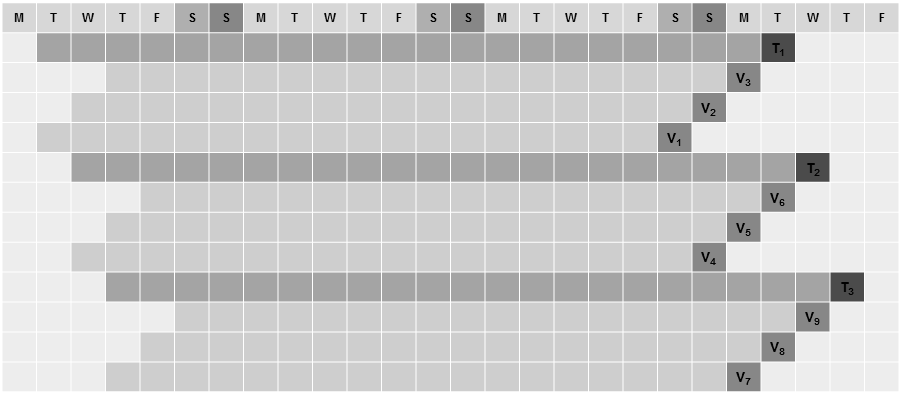
\includegraphics[width=.8\linewidth]{static/cross_validation_gray.png}
\end{center}

The training, validation, and test sets are defined as follows.
To exemplify the logic, we refer to Figure \ref{f:cv} that shows the calendar
    setup (i.e., weekdays on the x-axis) for three days $T_1$, $T_2$, and
    $T_3$ (shown in dark gray) for which we generate forecasts.
Each of these days is, by definition, a test day, and the test set comprises
    all time series, horizontal or vertical, whose last observation lies on
    that day.
With an assumed training horizon of three weeks, the 21 days before each of
    the test days constitute the corresponding training sets (shown in lighter
    gray on the same rows as $T_1$, $T_2$, and $T_3$).
There are two kinds of validation sets, depending on the decision to be made.
First, if a forecasting method needs parameter tuning, the original training
    set is divided into as many equally long series as validation days are
    needed to find stable parameters.
The example shows three validation days per test day named $V_n$ (shown
    in darker gray below each test day).
The $21 - 3 = 18$ preceding days constitute the training set corresponding to
    a validation day.
To obtain the overall validation error, the three errors are averaged.
We call these \textit{inner} validation sets because they must be repeated
    each day to re-tune the parameters and because the involved time series
    are true subsets of the original series.
Second, to find the best method per day and pixel, the same averaging logic
    is applied on the outer level.
For example, if we used two validation days to find the best method for $T_3$,
    we would average the errors of $T_1$ and $T_2$ for each method and select
    the winner; then, $T_1$ and $T_2$ constitute an \textit{outer} validation
    set.
Whereas the number of inner validation days is method-specific and must be
    chosen before generating any test day forecasts in the first place, the
    number of outer validation days may be varied after the fact and is
    determined empirically as we show in Section \ref{stu}.

Our unified CV approach is also optimized for large-scale production settings,
    for example, at companies like Uber.
As \cite{bell2018} note, there is a trade-off as to when each of the
    inner time series in the example begins.
While the forecasting accuracy likely increases with more training days,
    supporting inner series with increasing lengths, cutting the series
    to the same length allows caching the forecasts and errors.
In the example, $V_3$, $V_5$, and $V_7$, as well as $V_6$ and $V_8$ are
    identical despite belonging to different inner validation sets.
Caching is also possible on the outer level when searching for an optimal
    number of validation days for model selection.
We achieved up to 80\% cache hit ratios in our implementation in the
    empirical study, thereby saving computational resources by the same
    amount.
Lastly, we assert that our suggested CV, because of its being unified
    around whole test days and usage of fix-sized time series, is also
    suitable for creating consistent learning curves and, thus, answering
    \textbf{Q3} on the relationship between forecast accuracy and amount of
    historic data:
We simply increase the length of the outer training set holding the test day
    fixed.
Thus, independent of a method's need for parameter tuning, all methods have
    the same demand history available for each test day forecast.
